\documentclass[proposal,indonesia]{ugmskripsi}

%------------------------------------------------------------
% Metadata Proposal
%------------------------------------------------------------
\titleind{Perbandingan Terkontrol Paradigma \textit{Deployment} Manual dan GitOps dalam Menghadapi Penyimpangan Konfigurasi pada Klaster Kubernetes}
\titleeng{A Controlled Comparison of Manual and GitOps Deployment Paradigms in Responding to Configuration Drift on Kubernetes Clusters}
\fullname{Muhammad Argya Vityasy}
\idnum{23/522547/PA/22475}
\degree{Sarjana}
\gelar{S.Kom.}
\yearsubmit{2026}
\program{Ilmu Komputer}
\dept{Ilmu Komputer dan Elektronika}
\firstsupervisor{Guntur Budi Herwanto, S.Kom., M.Cs.}
\firstexaminer{Dr. techn. Kabul Kurniawan, S.Kom., M.Cs.}
\secondexaminer{Aina Musdholifah, S.Kom., M.Kom., Ph.D.}
\examdate{17 Juni 2026}

%------------------------------------------------------------
% Packages
%------------------------------------------------------------
\usepackage[utf8]{inputenc}
\usepackage{graphicx}
\graphicspath{{figures/}{diagrams/}}
\usepackage{amsmath}
\usepackage{amssymb}
\usepackage{booktabs}
\usepackage{longtable}
\usepackage{tabularx}
\usepackage{multirow}
\usepackage{float}
\usepackage{listings}
\usepackage{xcolor}
\usepackage{hyperref}
\usepackage{url}
\usepackage{xurl}
\usepackage{enumitem}
\usepackage{tikz}
\usetikzlibrary{shapes.geometric,arrows.meta,positioning,fit,backgrounds,calc}

\lstset{
    basicstyle=\ttfamily\small,
    breaklines=true,
    frame=single,
    numbers=left,
    numberstyle=\tiny,
    keywordstyle=\color{blue},
    commentstyle=\color{gray},
    stringstyle=\color{orange},
    showstringspaces=false,
    tabsize=2
}

\lstdefinelanguage{yaml}{
  keywords={true,false,null,y,n},
  sensitive=false,
  comment=[l]{\#},
  morecomment=[s]{/*}{*/},
  morestring=[b]',
  morestring=[b]"
}

\lstdefinelanguage{docker}{
  alsoletter={-},
  keywords={FROM,RUN,CMD,LABEL,MAINTAINER,EXPOSE,ENV,ADD,COPY,ENTRYPOINT,VOLUME,USER,WORKDIR,ARG,ONBUILD,STOPSIGNAL,HEALTHCHECK,SHELL},
  sensitive=false,
  comment=[l]{\#},
  morestring=[b]',
  morestring=[b]"
}

%------------------------------------------------------------
% Document Body
%------------------------------------------------------------
\begin{document}
\sloppy

\cover
\titlepageind
\approvalpage

\tableofcontents

\abstractind
Penelitian ini merancang evaluasi empiris terkontrol atas pengelolaan manual berbasis \texttt{kubectl} (Lingkungan A) dan GitOps berbasis ArgoCD (Lingkungan B) dalam menghadapi penyimpangan konfigurasi Kubernetes. Lingkungan A dijalankan oleh operator manusia dengan \textit{runbook} tetap dan diamati oleh \textit{observer}; pemeriksa kesetaraan bersifat \textit{read-only}. Beban formal adalah InvenioRDM nyata dengan sumber deployment yang dibekukan; surrogat historis tidak menjadi sampel formal. Kedua lengan dijalankan berurutan pada satu stack InvenioRDM karena kapasitas terverifikasi tidak mendukung dua stack serentak. Tujuh skenario direncanakan. Skenario A mempertahankan HPA normal pada kedua lengan sebagai kontrol respons HPA, bukan bukti efikasi ArgoCD; skenario F merupakan batas visibilitas objek di luar cakupan aplikasi. Keduanya dilaporkan terpisah dari drift terkelola B--E dan G. Metrik mencakup kesetaraan bidang konfigurasi (R1), waktu deteksi, ketersediaan bukti deviasi dan pemulihan konfigurasi (R2), serta bukti keterlacakan (R3). Waktu identifikasi akar masalah operasional pada lengan manual dicatat deskriptif dan tidak disamakan dengan bukti deviasi ArgoCD. Kesehatan dan adopsi runtime dinilai terpisah. Target deskriptif adalah lima pengulangan per skenario dan lengan untuk R1 serta sepuluh untuk R2, bukan jaminan daya uji. Waktu yang tidak teramati dicatat tersensor, bukan nol. Analisis eksploratif per skenario mempertimbangkan Mann--Whitney U dan ukuran efek untuk observasi lengkap yang sesuai. Rancangan masih menunggu tinjauan pemilik dan pembimbing; eksekusi formal dinonaktifkan, prasyarat kapasitas, audit, SMTP dan reset aplikasi belum terbukti, dan belum tersedia hasil komparatif formal.

\vspace{0.5cm}
\noindent\textbf{Kata Kunci:} penyimpangan konfigurasi, Kubernetes, GitOps, \textit{deployment} manual, evaluasi empiris terkontrol
\endabstractind

\abstracteng
This proposal designs a controlled empirical evaluation of manual kubectl management (Environment A) and GitOps using ArgoCD (Environment B) under Kubernetes configuration drift. Environment A is run by a human operator using a fixed runbook and observed live; the equality checker is read-only. The formal workload is real InvenioRDM with a frozen deployment source; historical surrogates are not formal samples. The two arms are executed sequentially on one InvenioRDM stack because verified capacity does not support two concurrent stacks. Seven scenarios are planned. Scenario A retains normal HPA operation in both arms as an HPA-response control, not evidence of ArgoCD efficacy; scenario F examines the visibility boundary for unmanaged objects. Both are reported separately from managed drift scenarios B--E and G. Metrics cover selected-field configuration equality (R1), detection, deviation-evidence availability and configuration recovery times (R2), and traceability evidence (R3). Operational root-cause identification time in the manual arm is recorded descriptively and is not equated with ArgoCD deviation evidence. Health and runtime adoption are assessed separately. Descriptive targets are five repetitions per scenario and arm for R1 and ten for R2, not a statistical-power guarantee. Unobserved times are censored rather than set to zero. Exploratory per-scenario analysis considers Mann--Whitney U and effect sizes for suitable complete observations. Methodological owner and supervisor review remains pending, formal execution is disabled, capacity, audit, SMTP and application-reset prerequisites remain unproven, and no formal comparative results are available.

\vspace{0.5cm}
\noindent\textbf{Keywords:} configuration drift, Kubernetes, GitOps, manual deployment, controlled empirical evaluation
\endabstracteng

%------------------------------------------------------------
% Chapters
%------------------------------------------------------------
\chapter{PENDAHULUAN}

\section{Latar Belakang}

Kubernetes telah menjadi platform \textit{container orchestration} yang dominan di industri maupun akademisi, digunakan oleh lebih dari 5,6 juta \textit{developer} secara global \citep{cncf2024}. Kemampuan Kubernetes dalam mengelola \textit{deployment}, \textit{scaling}, dan \textit{self-healing} menjadikannya pilihan utama untuk menjalankan aplikasi yang memerlukan \textit{availability} tinggi \citep{burns2016borg}. Namun, seiring bertambahnya jumlah layanan yang di-\textit{deploy} pada sebuah klaster, kompleksitas operasional meningkat secara drastis. Aplikasi yang dijalankan pada Kubernetes mencakup berbagai kelas \textit{workload} dengan karakteristik yang berbeda, antara lain: (1)~\textit{workload} web tanpa state (\textit{stateless web microservice}), (2)~\textit{workload} berbasis data yang menyimpan state (\textit{stateful data service}), serta (3)~\textit{workload} komposit multi-service yang terdiri atas banyak komponen yang saling bergantung \citep{siddiqui2023microservices, aghili2024workload}. Kelas terakhir, seperti platform data repositori skala besar, dapat terdiri dari 16 atau lebih komponen: layanan \textit{web}, \textit{worker} asinkron, \textit{database} relasional, \textit{search engine}, \textit{cache}, \textit{object storage}, \textit{ingress controller}, \textit{certificate manager}, enkripsi \textit{secret}, \textit{tunnel} jaringan, kebijakan keamanan, \textit{monitoring system}, dan \textit{backup}.

Pengelolaan \textit{deployment} aplikasi multi-service menggunakan pendekatan manual, yakni melalui perintah \texttt{kubectl apply}, \textit{manual scaling}, atau \textit{patching} langsung pada klaster, sering menghasilkan inkonsistensi operasional. Praktik ini rentan terhadap penyimpangan konfigurasi (\textit{configuration drift}), yaitu situasi di mana \textit{state} aktual klaster menyimpang dari \textit{state} yang didefinisikan secara deklaratif \citep{zhang2026configuration}. Penyimpangan konfigurasi dapat timbul akibat tiga penyebab utama: (1)~perubahan langsung pada klaster yang tidak tercatat dalam sistem \textit{version control}; (2)~prosedur \textit{deployment} yang tidak konsisten antar \textit{operator}; dan (3)~ketiadaan mekanisme deteksi otomatis yang dapat mengidentifikasi deviasi sebelum menimbulkan insiden.

Penelitian empiris oleh \citet{zhang2026configuration} menunjukkan bahwa 533 dari 719 \textit{defect} (74,1\%) menyebabkan \textit{crash}, operasi yang salah, atau \textit{outage}. \citet{rahman2023security} menambahkan bahwa \textit{security misconfiguration} pada manifest Kubernetes mencakup 11 kategori yang berulang, termasuk \textit{container} yang berjalan sebagai \textit{root} dan tanpa \textit{resource limits}. Temuan tersebut menunjukkan risiko konfigurasi, tetapi defect statis tidak identik dengan drift: penelitian ini membatasi intervensi pada perubahan terhadap acuan yang telah dibekukan.

GitOps menggunakan repositori Git sebagai \textit{source of truth} dan agen rekonsiliasi untuk menyelaraskan keadaan klaster \citep{opengitops2021}. Studi terdahulu telah membahas perbandingan konfigurasi deklaratif dan imperatif, waktu penanganan drift terhadap Ansible, serta rekonsiliasi GitOps dengan pembanding semiotomatis \citep{kaggantinataraja2025security,shrestha2024configuration,matubber2025managing}. Kebutuhan penelitian ini adalah bukti yang sesuai dengan konteks InvenioRDM, kepemilikan pengendali dan definisi pengukuran yang transparan, bukan klaim bahwa seluruh perbandingan terkontrol sebelumnya tidak ada.

Perbandingan tetap bermakna untuk mengukur besarnya perbedaan pada kondisi yang dicatat, bukan mengasumsikan GitOps unggul. Tekanan sumber daya, jadwal rekonsiliasi, hooks aplikasi dan pengendali lain dapat memengaruhi respons. Hasil operasional harus dikaitkan dengan konfigurasi serta batas pengamatan yang benar-benar digunakan \citep{forsgren2018accelerate}.

Kesenjangan tersebut menjadi landasan penelitian ini: mengevaluasi secara empiris kesetaraan konfigurasi (R1) serta waktu deteksi, ketersediaan bukti deviasi, dan pemulihan konfigurasi (R2) ketika tujuh skenario penyimpangan terjadi pada dua mode pengelolaan, yaitu imperatif terotomasi dan GitOps, pada satu stack InvenioRDM multi-service. Keterlacakan (R3) tidak diukur karena audit API server Kubernetes tidak tersedia; keterbatasan ini dinyatakan eksplisit. Hasil evaluasi mengkarakterisasi besaran dan kondisi perbedaan pada kasus yang diuji dan menjadi informasi kontekstual, bukan rekomendasi universal pemilihan paradigma.

\section{Rumusan Masalah}

Permasalahan yang dievaluasi adalah ketidaksetaraan konfigurasi terhadap acuan serta keterlambatan sinyal deteksi, ketersediaan bukti deviasi, dan pemulihan konfigurasi \citep{zhang2026configuration,rahman2023security,pohjola2025mitigating}. Status rollout sehat tidak menjamin konfigurasi cocok, dan riwayat Git tidak otomatis merekam pelaku mutasi di luar Git.

Pembanding pada rancangan ini adalah prosedur imperatif terotomasi tetap berbasis \texttt{kubectl}; pemeriksa dan \textit{runbook} otomatis membandingkan keadaan aktual dengan acuan dan menjalankan koreksi tanpa waktu reaksi manusia. Prosedur tersebut bukan \textit{deployment} terpisah: ia adalah mode pengelolaan pada stack InvenioRDM yang sama, dengan \textit{auto-sync} dan \textit{self-heal} ArgoCD dijeda sementara lalu dipulihkan. Mode GitOps menggunakan stack dan acuan yang sama dengan ArgoCD aktif. Kedua mode dijalankan berurutan; tidak ada eksekusi paralel A/B dan tidak ada stack kembar. Kepemilikan HPA normal tetap aktif pada kedua mode; respons replika HPA tidak dapat dijadikan bukti koreksi ArgoCD atas bidang yang diabaikannya.

Evaluasi mencakup dua pertanyaan: (1) bagaimana kesetaraan bidang konfigurasi berbeda setelah intervensi dan koreksi; serta (2) bagaimana waktu deteksi, ketersediaan bukti deviasi, dan waktu pemulihan konfigurasi berbeda. Tujuh skenario meliputi perubahan replika (A), image (B), ConfigMap (C), penghapusan objek (D), patch requests/limits (E), namespace salah (F), dan Secret (G). A dilaporkan sebagai kontrol HPA, F sebagai batas visibilitas objek tak terkelola, dan G sebagai kasus deskriptif yang bukan \textit{self-heal} ArgoCD; ketiganya tidak digabungkan ke estimasi efikasi B--E. Tidak adanya OutOfSync bukan deteksi nol; diff bukan identifikasi akar masalah. R3 tidak diukur karena audit API server tidak tersedia dan tidak dilaporkan sebagai nol atau tidak ada perbedaan.

\section{Batasan Masalah}

Agar penelitian tetap fokus dan terukur, batasan masalah yang ditetapkan adalah:

\begin{enumerate}
  \item Penelitian dilakukan pada klaster Kubernetes tunggal berbasis RKE2 dengan tiga \textit{node}, yaitu satu \textit{control-plane}/etcd dan dua \textit{worker}, yang menjalankan Kubernetes v1.32.6+rke2r1 pada Ubuntu 24.04 LTS; skenario \textit{multi-cluster} tidak termasuk dalam ruang lingkup.
  
  \item Beban formal adalah satu stack InvenioRDM nyata beserta dependensi multi-service di namespace \texttt{invenio}; sasaran sedikitnya 16 komponen memerlukan inventaris terverifikasi. Tidak ada stack kembar \texttt{exp-*} dan tidak ada surrogat pada desain formal; S1/S2 historis hanya artefak offline. Karena satu stack dipakai bergantian, beban latar dan dependensi bersama tidak dapat diisolasi dari perlakuan; inferensi dibatasi pada kasus dan apparatus yang benar-benar dicatat.
  
  \item Skenario penyimpangan konfigurasi yang diuji terbatas pada tujuh kategori: (A)~perubahan replika, (B)~perubahan \textit{image}, (C)~modifikasi ConfigMap, (D)~\textit{resource deletion}, (E)~\textit{patch} manual tidak sah, (F)~penyimpangan lintas \textit{namespace}, dan (G)~perubahan Secret.
  
  \item Dua mode pengelolaan dibandingkan pada satu stack: (a)~mode imperatif terotomasi menggunakan \texttt{kubectl} dengan pemeriksa dan \textit{runbook} otomatis, yang diperoleh dengan menjeda \textit{auto-sync}/\textit{self-heal} ArgoCD lalu memulihkannya; dan (b)~mode GitOps dengan ArgoCD aktif. HPA normal aktif pada keduanya. Mode dijalankan berurutan; tidak ada eksekusi paralel A/B dan tidak ada \textit{deployment} atau namespace kembar. Perubahan metodologis tetap draf untuk tinjauan pemilik dan pembimbing; eksekusi formal dinonaktifkan sampai seluruh gerbang kesiapan disetujui.
  
  \item Analisis statistik eksploratif menggunakan uji nonparametrik berpasangan/blok bila pemasangan dapat dipertahankan, atau \textit{Mann--Whitney U} dua sisi bila tidak, dengan tingkat signifikansi $\alpha = 0{,}05$ dan ukuran efek (Cohen's $d$, Cliff's $\delta$, atau Hodges--Lehmann) beserta interval kepercayaan. Waktu deteksi dan pemulihan yang tersensor kanan dianalisis dengan metode \textit{survival} (Kaplan--Meier); data tersensor dilaporkan terpisah dan tidak diimputasi sebagai nol. Observasi berurutan pada stack yang sama tidak diperlakukan independen secara naif.
  
  \item Paradigma perantara (Git sebagai \textit{source of truth} tanpa agen \textit{reconciliation} otomatis) dan paradigma \textit{push-based} (seperti Jenkins CI/CD atau Ansible yang mendorong perubahan ke klaster dari luar) tidak termasuk dalam ruang lingkup. Paradigma perantara tidak memiliki mekanisme koreksi otomatis sehingga tidak memenuhi prinsip GitOps \textit{continuous reconciliation}, sementara paradigma \textit{push-based} memerlukan kredensial klaster yang terekspos dan tidak memiliki \textit{feedback loop} bawaan \citep{utami2021analysis, shrestha2024configuration}. Keduanya merepresentasikan titik yang berbeda pada spektrum deklaratif-imperatif dan dapat dievaluasi pada penelitian lanjutan.

  \item R3 (bukti keterlacakan) tidak diukur karena audit API server Kubernetes tidak tersedia. Ketiadaan audit tidak menghambat \textit{deployment} atau pengukuran R1/R2; R3 dibahas sebagai keterbatasan dan pekerjaan lanjutan, bukan sebagai nol atau tidak ada perbedaan.
\end{enumerate}

\section{Tujuan Penelitian}

Tujuan penelitian adalah mengevaluasi perbedaan mode imperatif terotomasi dan GitOps pada kesetaraan konfigurasi (R1) serta waktu deteksi, ketersediaan bukti deviasi, dan pemulihan konfigurasi (R2) dalam konteks satu stack InvenioRDM. R3 tidak diukur karena audit API server tidak tersedia. Hasil tidak diasumsikan mendukung salah satu mode; kontrol HPA, batas visibilitas F, dan kasus deskriptif G tidak digabungkan menjadi klaim efikasi ArgoCD.

\section{Manfaat Penelitian}

Penelitian yang diuraikan dalam proposal ini diharapkan memberikan manfaat berikut:

\begin{enumerate}
  \item Teoritis: Memberikan bukti empiris terukur mengenai dampak operasional skenario penyimpangan konfigurasi pada dua paradigma \textit{deployment}, yang selama ini banyak didasarkan pada klaim \textit{vendor} atau studi kasus deskriptif. Hasil tersebut melengkapi literatur akademis dengan data eksperimental yang dapat direproduksi dan diverifikasi.
  
  \item Metodologis: Menawarkan protokol eksperimental yang dapat direplikasi, termasuk skenario penyimpangan terstandarisasi, metrik operasional, dan prosedur analisis statistik, sehingga penelitian selanjutnya dapat mereplikasi, memperluas, atau mengkritik temuan pada konteks dan platform yang berbeda.
  
  \item Praktis: Menyediakan bukti empiris terkontrol yang mengkarakterisasi perbedaan operasional antara kedua mode pengelolaan pada skenario penyimpangan yang diuji, serta menyoroti skenario yang paling rentan pada masing-masing mode, sehingga memberi informasi kontekstual bagi praktisi tanpa menjadi rekomendasi universal pemilihan paradigma.
\end{enumerate}

\section{Sistematika Penulisan}

Sistematika penulisan proposal tugas akhir ini adalah sebagai berikut:

\begin{itemize}
  \item Bab I: Pendahuluan, berisi latar belakang, rumusan masalah, batasan masalah, tujuan penelitian, manfaat penelitian, dan sistematika penulisan.
  \item Bab II: Penelitian Terkait, membahas studi empiris terkait penyimpangan konfigurasi pada Kubernetes, terminologi dasar, manajemen konfigurasi infrastruktur, paradigma \textit{deployment} alternatif, evaluasi GitOps dan ArgoCD, metode eksperimental pada riset sistem, serta \textit{research gap} yang menjadi landasan penelitian.
  \item Bab III: Metode dan Rancangan Penelitian, menjelaskan metodologi evaluasi empiris terkontrol, definisi variabel dan intervensi, tujuh skenario penyimpangan, protokol pengukuran, analisis statistik komparatif, ancaman terhadap validitas, dan lingkungan eksperimen.
  \item Bab IV: Jadwal Penelitian, memuat Gantt Chart berbasis bulan untuk perencanaan waktu penelitian selama 6 bulan.
\end{itemize}

\chapter{PENELITIAN TERKAIT}

\section{Penyimpangan Konfigurasi (\textit{Configuration Drift})}

Penyimpangan konfigurasi (\textit{configuration drift}) adalah situasi di mana \textit{state} aktual sebuah sistem menyimpang dari \textit{state} yang didefinisikan secara deklaratif \citep{rahman2020gang, hassan2024reconciliation}. Dalam konteks Kubernetes, penyimpangan terjadi ketika \textit{operator}, baik secara langsung maupun tidak sengaja, mengubah manifest klaster tanpa memperbarui \textit{source of truth} deklaratif, sehingga \textit{state} aktual dan \textit{desired state} menjadi tidak konsisten.

Penelitian empiris oleh \citet{zhang2026configuration} melakukan studi terhadap 719 \textit{defect} konfigurasi dari 2.260 skrip Kubernetes dan mengidentifikasi 15 kategori \textit{defect}, di mana 533 dari 719 \textit{defect} (74,1\%) menyebabkan \textit{crash}, operasi yang salah, atau \textit{outage}. Studi tersebut menegaskan bahwa \textit{misconfiguration} merupakan risiko operasional utama pada Kubernetes. \citet{rahman2023security} menambahkan bahwa \textit{security misconfiguration} pada manifest Kubernetes \textit{open-source} mencakup 11 kategori yang berulang, termasuk \textit{container} yang berjalan sebagai \textit{root}, tanpa \textit{drop capabilities}, dan tanpa \textit{resource limits}. Temuan tersebut didukung oleh \citet{rahman2019seven} yang mengidentifikasi tujuh \textit{security smells} berulang pada skrip IaC melalui studi empiris terhadap 1.726 skrip dan 15.232 skrip dari 293 repositori \textit{open-source}. Penelitian menunjukkan bahwa penyimpangan konfigurasi bukan hanya masalah estetika konfigurasi, tetapi ancaman nyata terhadap keandalan dan keamanan layanan.

\citet{rahman2020gang} memberikan taksonomi empiris untuk memahami sumber dan dampak penyimpangan pada sistem \textit{Infrastructure-as-Code} (IaC). Melalui analisis kualitatif terhadap 1.448 \textit{commit} terkait \textit{defect} dan kuantifikasi terhadap 80.425 \textit{commit} dari 291 repositori, penelitian tersebut mengidentifikasi delapan kategori \textit{defect}, di mana kategori data konfigurasi yang keliru merupakan kategori paling sering muncul dan kategori \textit{idempotency} merupakan kategori khas IaC yang paling disepakati oleh 66 praktisi yang disurvei. Taksonomi tersebut menyediakan dasar empiris untuk mengoperasionalkan faktor pendorong penyimpangan pada R1, menggantikan kerangka konseptual tanpa validasi Kubernetes-eksklusif.

\subsection{Faktor yang Menimbulkan Penyimpangan Konfigurasi}

Berdasarkan literatur, faktor-faktor utama yang memperburuk penyimpangan konfigurasi pada Kubernetes meliputi:

\begin{enumerate}
  \item Perubahan langsung pada klaster: Penggunaan \texttt{kubectl\allowbreak{} edit}, \texttt{kubectl\allowbreak{} patch}, atau \texttt{kubectl\allowbreak{} scale} secara langsung tanpa memperbarui repositori \textit{source of truth} \citep{zhang2026configuration}.
  
  \item Prosedur \textit{deployment} yang tidak terdokumentasi: Setiap \textit{operator} dapat memiliki urutan perintah yang berbeda, yang mengakibatkan \textit{state} klaster tidak deterministik \citep{rahman2020gang}.
  
  \item Kurangnya mekanisme \textit{rollback} yang terintegrasi: \textit{Deployment} manual seringkali tidak memiliki mekanisme \textit{rollback} otomatis; \textit{operator} harus mengingat konfigurasi sebelumnya atau mengandalkan \textit{backup} yang mungkin tidak konsisten \citep{rahman2023security, rahman2019seven}.
  
  \item Ketiadaan mekanisme deteksi penyimpangan otomatis: Tanpa pemeriksaan berkala antara \textit{state} aktual dan \textit{desired state}, penyimpangan dapat terakumulasi selama periode lama tanpa terdeteksi \citep{zhang2026configuration}.
\end{enumerate}

\section{Terminologi Dasar}

Bagian ini mendefinisikan terminologi kunci yang digunakan dalam penelitian, dengan tujuan membangun dasar konseptual yang konsisten sebelum pembahasan lebih lanjut.

\subsection{Kubernetes dan Orkestrasi Kontainer}
Kubernetes adalah platform \textit{container orchestration} \textit{open-source} yang mengotomasi \textit{deployment}, \textit{scaling}, dan manajemen aplikasi terkemas (\textit{containerized}) \citep{burns2016borg}. Kubernetes awalnya dikembangkan oleh Google berdasarkan pengalaman mengelola sistem \textit{workload} berskala besar di Borg dan Omega, dan kini menjadi standar de facto untuk orkestrasi kontainer di industri \citep{verma2015borg}. Pada Kubernetes, \textit{state} yang diinginkan (\textit{desired state}) dideklarasikan melalui berkas konfigurasi (\textit{manifest}), dan \textit{control plane} bertanggung jawab mencapai dan mempertahankan \textit{state} tersebut.

\subsection{Git dan \textit{Version Control}}
Git adalah sistem \textit{version control} terdistribusi yang merekam setiap perubahan pada berkas beserta metadata (penulis, \textit{timestamp}, pesan \textit{commit}) \citep{chacon2014git}. Dalam konteks GitOps, Git berfungsi sebagai \textit{single source of truth} yang menyimpan deklarasi \textit{state} infrastruktur dan aplikasi, sehingga setiap perubahan dapat dilacak, di-\textit{review}, dan dikembalikan (\textit{rollback}) secara andal.

\subsection{\textit{Continuous Integration} dan \textit{Continuous Deployment}}
\textit{Continuous Integration} (CI) adalah praktik di mana perubahan kode secara otomatis diuji dan digabungkan ke \textit{branch} utama, sementara \textit{Continuous Deployment} (CD) adalah perluasan CI di mana perubahan yang lulus pengujian secara otomatis di-\textit{deploy} ke lingkungan produksi tanpa intervensi manual eksplisit \citep{humble2010continuous, ebert2016devops}. GitOps merupakan paradigma spesifik di dalam CD yang menggunakan repositori Git sebagai \textit{single source of truth}.

\subsection{\textit{Infrastructure-as-Code} (IaC)}
\textit{Infrastructure-as-Code} (IaC) adalah praktik mendefinisikan dan mengelola infrastruktur melalui berkas konfigurasi yang diberi versi (\textit{versioned}), bukan melalui proses manual \citep{morris2020iac}. IaC memungkinkan \textit{version control}, \textit{code review}, dan reprodusibilitas lingkungan. Dalam konteks Kubernetes, IaC diimplementasikan melalui \textit{manifest} deklaratif (YAML) yang mendefinisikan \textit{desired state} klaster.

\subsection{Paradigma Deklaratif vs Imperatif}
Dalam paradigma imperatif, \textit{operator} memberikan serangkaian perintah langkah demi langkah yang mengubah \textit{state} sistem secara langsung (\textit{how to achieve the state}). Dalam paradigma deklaratif, \textit{operator} mendefinisikan \textit{desired state} dan sistem bertanggung jawab mencapai serta mempertahankan \textit{state} tersebut (\textit{what state to achieve}) \citep{scott2015plp}. Perbedaan fundamental ini memiliki implikasi langsung terhadap bagaimana sistem merespons deviasi konfigurasi: paradigma deklaratif mendukung \textit{convergence} otomatis, sementara paradigma imperatif memerlukan intervensi manual eksplisit untuk setiap deviasi.

\section{Manajemen Konfigurasi Infrastruktur}

\textit{Infrastructure state management} adalah disiplin yang mengatur bagaimana \textit{state} sebuah sistem infrastruktur didefinisikan, diterapkan, dan dipertahankan. Dalam paradigma deklaratif, \textit{operator} mendefinisikan \textit{desired state} melalui konfigurasi yang telah dibakukan (\textit{Infrastructure-as-Code}), dan sistem bertanggung jawab untuk mencapai serta mempertahankan \textit{state} tersebut \citep{morris2020iac}. Dalam paradigma imperatif, \textit{operator} memberikan serangkaian perintah langkah demi langkah yang mengubah \textit{state} sistem secara langsung \citep{limoncelli2018}. Perbedaan fundamental ini memiliki implikasi langsung terhadap bagaimana sistem merespons deviasi konfigurasi: paradigma deklaratif mendukung \textit{convergence} otomatis, sementara paradigma imperatif memerlukan intervensi manual untuk setiap deviasi.

\section{\textit{Continuous Deployment} dan Paradigma GitOps}

\textit{Continuous Deployment} (CD) adalah praktik dalam ranah DevOps di mana setiap perubahan kode yang lulus pengujian secara otomatis di-\textit{deploy} ke lingkungan produksi tanpa intervensi manual eksplisit \citep{limoncelli2018, ebert2016devops}. CD merupakan perluasan dari \textit{Continuous Integration} (CI) dan bertujuan meminimalkan waktu antara penulisan kode dan ketersediaannya bagi pengguna akhir. Dalam ekosistem Kubernetes, CD memerlukan mekanisme yang dapat secara andal menyelaraskan perubahan konfigurasi dengan \textit{state} klaster.

GitOps adalah paradigma spesifik di dalam CD yang menggunakan repositori Git sebagai \textit{single source of truth} untuk mendefinisikan \textit{state} infrastruktur dan aplikasi. CNCF GitOps Working Group mendefinisikan empat prinsip OpenGitOps: (1)~sistem dideklarasikan secara deklaratif; (2)~\textit{state} sistem yang diinginkan tersimpan dan diberi versi (\textit{versioned}) dalam Git; (3)~perubahan \textit{state} ditarik (\textit{pulled}) secara otomatis oleh agen \textit{software}; dan (4)~agen \textit{software} secara kontinu mendeteksi dan mengoreksi deviasi dari \textit{state} yang diinginkan \citep{opengitops2021}.

Karakteristik GitOps yang berbeda dari pendekatan imperatif tradisional meliputi: \textit{audit trail} lengkap melalui Git \textit{history}, penerapan \textit{code review} pada perubahan infrastruktur, \textit{rollback} yang sederhana melalui \texttt{git revert}, dan reprodusibilitas konfigurasi di berbagai lingkungan \citep{yuen2021gitops}. Dalam model \textit{pull-based} GitOps, agen yang berjalan di dalam klaster secara periodik membandingkan \textit{state} Git dengan \textit{state} klaster dan menyelaraskan keduanya, menghilangkan kebutuhan akan akses kredensial klaster dari luar \citep{utami2021analysis}.

\subsection{Performa \textit{Deployment} dan \textit{Anti-Pattern}}

Forsgren dkk. \citep{forsgren2018accelerate} mengidentifikasi empat metrik kunci yang mengkarakterisasi performa \textit{deployment} pada organisasi teknologi: (1)~\textit{deployment frequency}, (2)~\textit{lead time for changes}, (3)~\textit{time to restore service}, dan (4)~\textit{change failure rate}. Operasionalisasi keempat metrik tersebut untuk pengukuran otomatis dibahas oleh \citet{sallin2021measuring} melalui prototipe pengukuran otomatis pada XP 2021, sementara \citet{wilkes2023framework} memformalkan kerangka pengukuran DORA yang independen terhadap siklus hidup pengembangan dan memvalidasinya pada 304 repositori \textit{open-source}, sehingga mendukung justifikasi pengumpulan metrik berbasis \textit{polling} dalam penelitian ini. Metrik-metrik tersebut menunjukkan bahwa organisasi yang mengadopsi praktik \textit{continuous deployment} dan \textit{Infrastructure-as-Code} secara konsisten mengungguli organisasi yang bergantung pada proses manual. Lebih lanjut, praktik \textit{deployment} manual yang mengabaikan \textit{version control} dan \textit{automated reconciliation} merupakan \textit{anti-pattern} yang berkontribusi terhadap penyimpangan konfigurasi \citep{beyer2016sre}. Dalam konteks penelitian yang diuraikan dalam proposal ini, metrik \textit{time to restore service} dan \textit{change failure rate} berelasi langsung dengan metrik R2 (waktu deteksi/pemulihan) dan R1 (konsistensi \textit{deployment}) yang digunakan dalam eksperimen.

ArgoCD mengimplementasikan prinsip-prinsip GitOps melalui \textit{reconciliation loop} yang berjalan di dalam klaster. ArgoCD terdiri dari tiga komponen utama: (1)~\textit{application controller} yang secara periodik membandingkan \textit{state} Git dengan \textit{state} aktual dan melakukan tindakan korektif; (2)~\textit{repo server} yang mengelola koneksi ke repositori Git; dan (3)~\textit{Redis cache} yang menyimpan \textit{state} sementara untuk performa \citep{argocd2024}. ArgoCD berperan sebagai \textit{negative feedback controller}: setiap deviasi (penyimpangan) bersifat \textit{transien}, yaitu sistem secara otomatis kembali ke \textit{desired state} tanpa memerlukan intervensi manusia, sepanjang \textit{self-heal} diaktifkan.

\section{Dasar Teori: \textit{Reconciliation} dan \textit{Convergence} pada Sistem Deklaratif}

Karakteristik GitOps yang berbeda dari pendekatan imperatif dapat dijelaskan melalui dua prinsip teoretis yang saling berkaitan.

\subsection{\textit{Convergence} Menuju \textit{Desired State}}

Konsep \textit{negative feedback controller} menjelaskan upaya sistem mencapai keadaan yang diinginkan \citep{limoncelli2018}. ArgoCD membandingkan deklarasi dengan keadaan klaster dan dapat mengoreksi perbedaan sesuai kebijakan, izin dan cakupannya \citep{argocd2024,hassan2024reconciliation}. Hal ini tidak menjamin setiap perubahan ditemukan atau pulih: bidang yang diabaikan, objek tak terkelola, kegagalan pengendali dan kepemilikan HPA membatasi interpretasi. Pada rancangan ini, respons replika HPA dipisahkan dari self-heal ArgoCD.

Perintah imperatif tidak dengan sendirinya menyediakan rekonsiliasi berkelanjutan, tetapi pemeriksaan dan koreksinya dapat diotomasi \citep{hassan2024reconciliation,rahman2020gang}. Pembanding penelitian ini menggunakan prosedur imperatif terotomasi tetap; pemeriksa dan runbook berjalan otomatis tanpa waktu reaksi manusia. Waktu reaksi manusia tidak dimasukkan sebagai variabel.

\subsection{\textit{Audit Trail} sebagai \textit{Social Control Mechanism}}

Git merekam perubahan deklarasi yang dikomit beserta metadata dan dapat mendukung peninjauan perubahan \citep{opengitops2021}. Mutasi langsung pada klaster tidak otomatis masuk riwayat Git. Bukti audit API dan tindakan pengendali tetap diperlukan untuk merekonstruksi pelaku, urutan dan hasil mutasi; kelengkapannya dinilai, bukan diasumsikan.

\section{\textit{Runbook} sebagai Standarisasi Prosedur Pemulihan}

\textit{Runbook} adalah dokumen terstandarisasi yang berisi prosedur operasional untuk menanggapi insiden atau melakukan pemulihan (\textit{recovery}) pada sebuah sistem. Dalam ranah operasi TI, \textit{runbook} berfungsi sebagai \textit{playbook} yang mendefinisikan langkah-langkah korektif berurutan berdasarkan jenis insiden, sehingga setiap \textit{operator} yang berbeda mengikuti urutan tindakan yang sama \citep{schlette2024playbook}. Penggunaan \textit{runbook} mengurangi variabilitas akibat keahlian \textit{operator} yang berbeda-beda dan memastikan bahwa keputusan subjektif diminimalkan selama pemulihan.

Pada rancangan ini, runbook merupakan prosedur koreksi otomatis berdasarkan perbedaan yang teramati, tanpa menerima label skenario dari injector. Entry point \texttt{recovery-runbook.sh} saat ini memvalidasi bukti hasil koreksi dan reset secara offline. Eksekusi langsung tetap dinonaktifkan sampai integrasi lifecycle dan postcondition disetujui. Selesainya diagnosis atau rollout sehat bukan bukti seluruh konfigurasi maupun data aplikasi telah pulih.

\section{Paradigma \textit{Deployment} Alternatif}

Selain paradigma manual dan GitOps yang menjadi fokus penelitian yang diuraikan dalam proposal ini, terdapat paradigma \textit{deployment} lain yang menempati posisi berbeda pada spektrum deklaratif-imperatif. Pertama, paradigma \textit{push-based} \textit{Continuous Deployment} (misalnya Jenkins CI/CD) mendorong perubahan dari luar klaster ke dalam klaster melalui \textit{pipeline} otomatis. Meskipun menawarkan otomasi \textit{deployment}, paradigma ini memerlukan kredensial klaster yang terekspos pada \textit{pipeline} eksternal dan tidak memiliki mekanisme \textit{reconciliation} bawaan: ketika \textit{state} klaster menyimpang, \textit{pipeline} tidak secara aktif mendeteksi atau mengoreksi deviasi \citep{utami2021analysis}. Kedua, manajemen konfigurasi imperatif menggunakan alat seperti Ansible atau Terraform menerapkan perubahan melalui perintah imperatif yang dijalankan dari luar klaster. \citet{shrestha2024configuration} mengevaluasi Ansible sebagai alternatif GitOps dan menemukan bahwa meskipun Ansible menyediakan otomasi \textit{deployment}, ia tidak memiliki \textit{continuous reconciliation} dan \textit{audit trail} bawaan yang dimiliki GitOps. Ketiga, paradigma perantara --- Git sebagai \textit{source of truth} tanpa agen \textit{reconciliation} otomatis --- merepresentasikan titik di mana deklarasi \textit{state} disimpan dalam Git, tetapi koreksi penyimpangan tetap bergantung pada intervensi manual.

Perbandingan difokuskan pada prosedur imperatif terotomasi terstandarisasi dan ArgoCD dengan konfigurasi yang dicatat. Tidak ada klaim bahwa selisihnya menjadi batas atas seluruh alternatif. HPA normal pada kedua lengan merupakan pengendali bersama, bukan perbedaan paradigma.

\section{Evaluasi Empiris GitOps dan ArgoCD}

\citet{utami2021analysis} melakukan analisis perbandingan model \textit{deployment} deklaratif \textit{pull-based} (GitOps dengan ArgoCD) versus \textit{push-based} pada Kubernetes, dan menemukan bahwa model \textit{pull-based} dilaporkan lebih andal karena agen berjalan di dalam klaster dan tidak memerlukan kredensial eksternal. \citet{shrestha2024configuration} mengevaluasi GitOps versus Ansible untuk manajemen konfigurasi Kubernetes, termasuk waktu induksi, penemuan, dan penanganan drift; pembanding Ansible dan konteks protokolnya berbeda dari prosedur imperatif tetap serta kepemilikan pengendali yang dirancang di sini. \citet{kaggantinataraja2025security} melakukan analisis berpusat keamanan terhadap pendekatan deklaratif (GitOps/ArgoCD) dan imperatif (Jenkins/\texttt{kubectl}) pada Minikube satu node dengan konfigurasi keamanan yang berbeda, dan melaporkan koreksi penyimpangan yang lebih cepat, \textit{compliance rate} yang lebih tinggi, serta paparan kerentanan yang lebih rendah. Skala satu node dan perbedaan konfigurasi tersebut membatasi transfer temuan ke klaster multi-node dan apparatus penelitian ini.

Di sisi fondasi empiris IaC, \citet{hassan2024reconciliation} mengkategorikan 5.110 \textit{defect} rekonsiliasi \textit{state} ke dalam delapan kategori sebagai landasan teori \textit{reconciliation loop}, sementara \citet{rahman2019properties} mengidentifikasi 10 properti kode sumber yang berkorelasi dengan skrip IaC yang cacat dan mendukung pemilihan uji \textit{Mann--Whitney} beserta ukuran efek Cliff's Delta. \citet{matubber2025managing} mengukur \textit{reconciliation time}, \textit{scalability}, dan \textit{reliability} GitOps untuk infrastruktur K8s, termasuk \textit{self-healing} terhadap penyimpangan konfigurasi; pembandingnya berupa alur kerja lama yang semi-terotomasi, bukan prosedur imperatif tetap dengan acuan dan kepemilikan pengendali yang sama seperti rancangan ini.

Tabel~\ref{tab:literatur-comparison} merangkum kelemahan metodologis kunci dari penelitian-penelitian tersebut.

\begin{table}[H]
  \centering
  \small
  \caption{Perbandingan Kelemahan Metodologis Penelitian Terdahulu}
  \label{tab:literatur-comparison}
  \begin{tabular}{|>{\raggedright\arraybackslash}p{3.4cm}|>{\raggedright\arraybackslash}p{3.2cm}|>{\raggedright\arraybackslash}p{5.8cm}|}
    \hline
    Penelitian & Fokus & Kelemahan Metodologis \\
    \hline
    \citet{shrestha2024configuration} & GitOps vs Ansible & Penilaian kualitatif untuk tingkat keparahan penyimpangan; rincian uji formal tidak dinilai dalam ringkasan ini \\
    \hline
    \citet{kaggantinataraja2025security} & Keamanan deklaratif vs imperatif & Minikube satu node dan konfigurasi keamanan berbeda membatasi transfer konteks \\
    \hline
    \citet{matubber2025managing} & \textit{Reconciliation time} GitOps & Pembanding legacy semiotomatis bukan prosedur imperatif tetap penelitian ini \\
    \hline
  \end{tabular}
\end{table}

\section{Metode Eksperimental Terkontrol pada Riset Sistem}

Evaluasi empiris pada riset sistem dan infrastruktur memerlukan desain eksperimental yang memitigasi ancaman terhadap validitas \citep{wohlin2012experimentation}. \citet{limoncelli2018} menjelaskan bahwa penelitian sistem harus membangun lingkungan yang dapat direproduksi, mengendalikan variabel pengganggu, dan mendefinisikan metrik yang jelas sebelum menyimpulkan hubungan kausal.

Rancangan membandingkan dua prosedur dengan intervensi dan acuan setara serta kendali pengganggu yang didokumentasikan \citep{wohlin2012experimentation}. Pengendalian tersebut tidak menjamin paradigma abstrak menjadi satu-satunya perbedaan; jadwal, implementasi pengendali dan kepemilikan bidang tetap membatasi inferensi.

Analisis eksploratif dapat menggunakan Mann--Whitney U dan ukuran efek untuk waktu teramati lengkap dengan asumsi yang sesuai \citep{wohlin2012experimentation,rahman2019properties}. Data tersensor tidak boleh diubah menjadi waktu sukses atau diam-diam dibuang; aturan analisis dan target pengulangan dijelaskan pada Bab III. A dan F tetap terpisah dari efikasi ArgoCD.

\section{Klasifikasi Beban Uji (\textit{Workload})}

Aplikasi yang dijalankan pada klaster Kubernetes dapat dikelompokkan ke dalam beberapa kelas \textit{workload} berdasarkan karakteristik arsitektur dan manajemen \textit{state} \citep{siddiqui2023microservices, aghili2024workload}:

\begin{enumerate}
  \item \textit{Workload} web tanpa state (\textit{stateless web microservice}): Layanan yang tidak menyimpan \textit{state} secara internal, sehingga setiap permintaan dapat dilayani oleh instans mana pun. Contoh: server HTTP sederhana, \textit{API gateway}.
  
  \item \textit{Workload} berbasis data yang menyimpan \textit{state} (\textit{stateful data service}): Layanan yang menyimpan \textit{state} secara persisten, seperti \textit{database} relasional, \textit{search engine}, atau \textit{object storage}. \textit{Workload} kelas ini memerlukan urutan \textit{deployment} dan penanganan penyimpangan yang lebih kompleks.
  
  \item \textit{Workload} komposit multi-service: Aplikasi yang terdiri atas banyak komponen yang saling bergantung, mencakup kombinasi kelas 1 dan 2 beserta komponen infrastruktur (\textit{ingress}, TLS, \textit{secrets}, \textit{monitoring}, \textit{backup}, kebijakan keamanan). Kelas \textit{workload} ini memiliki kompleksitas dependensi tertinggi dan paling rentan terhadap penyimpangan konfigurasi akibat banyaknya komponen yang harus diselaraskan.
\end{enumerate}

Beban formal penelitian adalah InvenioRDM nyata, meliputi web, worker/scheduler, PostgreSQL, OpenSearch, Redis, penyimpanan persisten dan infrastruktur pendukung. Sasaran cakupan sedikitnya 16 komponen memerlukan inventaris dari sumber deployment dan keadaan aktual; daftar konseptual bukan bukti jumlah komponen atau penggunaan MinIO/S3 oleh aplikasi. Beban uji merupakan apparatus studi empiris, bukan produk yang dikembangkan. Temuan dibatasi pada konfigurasi InvenioRDM yang benar-benar digunakan; NGINX S1/S2 historis tidak menjadi pengganti atau dasar generalisasi formal.

\section{Kesenjangan Penelitian (\textit{Research Gap})}

Berdasarkan tinjauan pustaka yang telah diuraikan, terdapat empat kesenjangan yang saling berkaitan dan menjadi landasan penelitian:

\begin{enumerate}
  \item Kesenjangan Validitas Konstruk: Studi terdahulu memakai definisi penyimpangan, metrik, dan cakupan yang berbeda. \citet{shrestha2024configuration} memakai penilaian kualitatif untuk tingkat keparahan, sedangkan \citet{kaggantinataraja2025security} berfokus pada keamanan dan \textit{compliance rate}. Perbedaan operasionalisasi tersebut membatasi perbandingan langsung dengan kesetaraan bidang, kesehatan, dan bukti deviasi yang didefinisikan dalam rancangan ini.

  \item Kesenjangan Validitas Internal: Konfigurasi apparatus, skala klaster, pembanding, dan kepemilikan pengendali berbeda antarstudi. \citet{kaggantinataraja2025security} memakai Minikube satu node dengan konfigurasi keamanan berbeda, sedangkan \citet{matubber2025managing} memakai pembanding legacy semiotomatis. Perbedaan tersebut membatasi transfer atribusi kausal ke konteks InvenioRDM dengan HPA normal pada kedua lengan.

  \item Kesenjangan Metodologis: Belum ditemukan evaluasi yang menggunakan kontrak bidang konfigurasi yang sama pada kedua lengan, memisahkan sinyal pengendali dari rollout, serta mempertahankan hasil tersensor dan kegagalan reset pada beban InvenioRDM ini. Rancangan ini ditujukan untuk mengisi kebutuhan tersebut; klaim mengenai hasilnya menunggu data formal.

  \item Kesenjangan Kontekstual: Evaluasi GitOps yang ada dilakukan pada konteks dan protokol yang bervariasi. Belum ditemukan evaluasi terkontrol pada apparatus InvenioRDM nyata dengan dependensi multi-service, kepemilikan HPA, serta pemisahan skenario kontrol, drift terkelola, dan batas visibilitas seperti yang dirancang di sini.
\end{enumerate}

Rancangan ini ditujukan untuk mengoperasionalisasi R1/R2 dan rubrik deskriptif R3 dalam konteks tersebut, dengan pengendalian sumber serta pengukuran yang dapat diperiksa. Kontribusi empiris dan besarnya perbedaan baru dapat dinilai setelah metode ditinjau, apparatus divalidasi, dan data formal dikumpulkan.

\chapter{METODE DAN RANCANGAN PENELITIAN}

\section{Deskripsi Umum dan Status Rancangan}

Penelitian ini merancang evaluasi empiris terkontrol atas pengelolaan imperatif terotomasi berbasis \texttt{kubectl} (Lingkungan A, disebut manual dalam judul) dan GitOps berbasis ArgoCD (Lingkungan B). Beban formal adalah InvenioRDM nyata beserta dependensi multi-service, bukan aplikasi NGINX pengganti. Yang dibandingkan adalah dua prosedur operasional pada konfigurasi tertentu, bukan keunggulan universal suatu paradigma.

Revisi metodologis ini merupakan draf untuk tinjauan pemilik penelitian dan pembimbing. Eksperimen formal belum disetujui dan eksekusi langsung instrumen dinonaktifkan. Kelulusan uji offline tidak membuktikan kesiapan klaster, audit, SMTP, kapasitas, ataupun pemulihan data aplikasi. Proposal yang diterima sebelumnya dan artefak historis tetap dapat ditelusuri melalui riwayat versi; perubahan definisi tidak mengubah makna hasil historis menjadi hasil formal.

\section{Metodologi dan Kesetaraan Perbandingan}

Rancangan mengikuti evaluasi empiris terkontrol dengan pengamatan kondisi dasar, satu intervensi, dan pengamatan pascaintervensi \citep{wohlin2012experimentation}. Kedua lingkungan dibangun secara sengaja pada satu klaster; rancangan bukan penugasan acak klaster dari populasi \citep{cook1979quasi}. Unit analisis adalah satu injeksi yang diterima pada satu lingkungan dalam satu pengulangan.

Kedua lingkungan menggunakan sumber deployment, image digest, inventaris, kontrak bidang konfigurasi, kebijakan HPA, dan aturan pengukuran yang setara. Lingkungan manual berada di luar kepemilikan ArgoCD. Urutan lingkungan dan skenario diacak dalam blok; hanya satu injeksi diperbolehkan setelah reset sebelumnya terverifikasi. Tidak ada eksekusi semua mutasi tanpa reset di antaranya.

Pemeriksa imperatif membandingkan keadaan aktual dengan acuan yang dibekukan, menyimpan bukti perbedaan, lalu menjalankan koreksi tetap. Tidak ada penundaan untuk reaksi atau pengetikan manusia. Identitas skenario tidak diberikan kepada mekanisme koreksi. Peneliti membakukan prosedur dan meninjau bukti, bukan menjadi subjek pengukuran kinerja manusia; NASA-TLX dan waktu identifikasi akar masalah manusia tidak menjadi metrik rancangan ini. Prosedur pemulihan tetap mengikuti prinsip runbook yang dapat diperiksa \citep{schlette2024playbook}.

\begin{figure}[H]
  \centering
  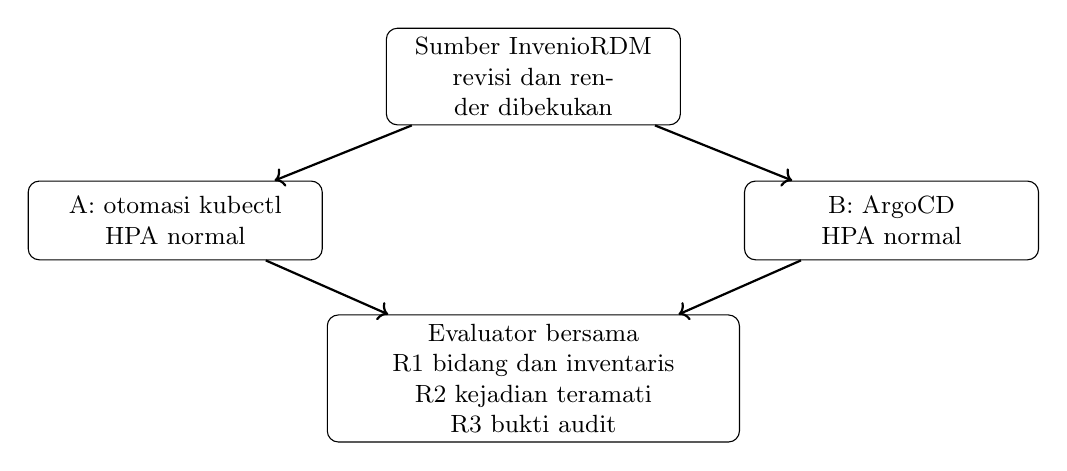
\begin{tikzpicture}[
    box/.style={draw, rounded corners, align=center, text width=3.5cm, minimum height=10mm, font=\small},
    flow/.style={->, thick}, node distance=7mm and 8mm]
    \node[box] (source) {Sumber InvenioRDM\\revisi dan render dibekukan};
    \node[box, below left=of source] (manual) {A: otomasi kubectl\\HPA normal};
    \node[box, below right=of source] (gitops) {B: ArgoCD\\HPA normal};
    \node[box, below=24mm of source, text width=5cm] (measure) {Evaluator bersama\\R1 bidang dan inventaris\\R2 kejadian teramati\\R3 bukti audit};
    \draw[flow] (source) -- (manual);
    \draw[flow] (source) -- (gitops);
    \draw[flow] (manual) -- (measure);
    \draw[flow] (gitops) -- (measure);
  \end{tikzpicture}
  \caption{Rancangan apparatus dengan HPA aktif pada kedua lingkungan.}
  \label{fig:arsitektur-eksperimen}
\end{figure}

Gambar~\ref{fig:arsitektur-eksperimen} membedakan mekanisme deployment dari evaluator. HPA merupakan pengendali bersama, sehingga responsnya tidak diatribusikan kepada ArgoCD.

\begin{figure}[H]
  \centering
  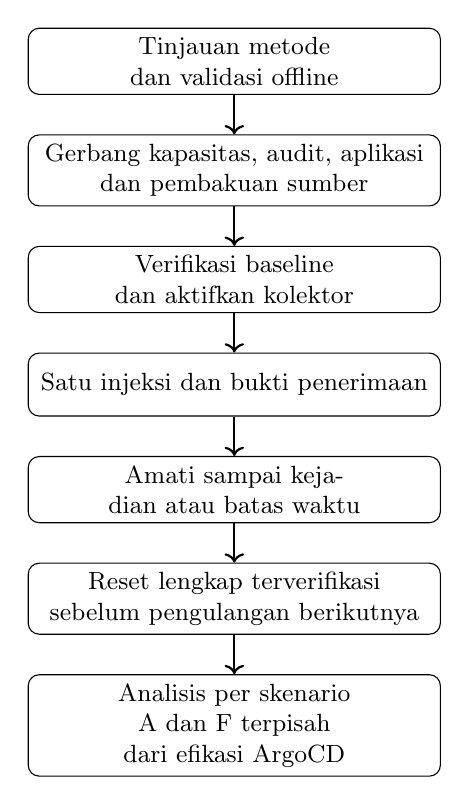
\begin{tikzpicture}[
    box/.style={draw, rounded corners, align=center, text width=5cm, minimum height=8mm, font=\small},
    flow/.style={->, thick}, node distance=5mm]
    \node[box] (review) {Tinjauan metode dan validasi offline};
    \node[box, below=of review] (ready) {Gerbang kapasitas, audit, aplikasi\\dan pembakuan sumber};
    \node[box, below=of ready] (baseline) {Verifikasi baseline dan aktifkan kolektor};
    \node[box, below=of baseline] (inject) {Satu injeksi dan bukti penerimaan};
    \node[box, below=of inject] (observe) {Amati sampai kejadian atau batas waktu};
    \node[box, below=of observe] (reset) {Reset lengkap terverifikasi\\sebelum pengulangan berikutnya};
    \node[box, below=of reset] (analysis) {Analisis per skenario\\A dan F terpisah dari efikasi ArgoCD};
    \draw[flow] (review) -- (ready);
    \draw[flow] (ready) -- (baseline);
    \draw[flow] (baseline) -- (inject);
    \draw[flow] (inject) -- (observe);
    \draw[flow] (observe) -- (reset);
    \draw[flow] (reset) -- (analysis);
  \end{tikzpicture}
  \caption{Bagan alir rancangan penelitian; pelaksanaan formal tetap menunggu persetujuan.}
  \label{fig:bagan-alir-eksperimen}
\end{figure}

Gambar~\ref{fig:bagan-alir-eksperimen} menempatkan gerbang kesiapan sebelum injeksi. Kegagalan dan data tersensor disimpan, bukan dihapus agar hanya pemulihan sukses yang dilaporkan.

\section{Lingkungan dan Provenans Deployment}

Konteks deployment yang dilaporkan pemilik adalah tiga node, 24 inti CPU, sekitar 23 Gi memori, Kubernetes 1.32.6 dengan RKE2/containerd, dan Ubuntu 24.04. Nilai ini menggantikan target lama Kubernetes 1.29+ dan Ubuntu 22.04; bukan hasil pemeriksaan live baru dalam revisi ini. Sebelum pengumpulan formal, versi runtime, alokasi node, dan revisi yang benar-benar diterapkan harus direkam ulang.

Sumber otoritatif adalah repositori \url{https://github.com/vityasyyy/invenio-rdm-gitops}. Revisi referensi yang diperiksa ialah \nolinkurl{6cacea6642a7c1690243d3b54130fa08216a9595}; penunjuknya disimpan pada \path{experiments/deployment-source.json}. Application \path{argocd/apps/invenio-bootstrap.yaml} memilih \path{k8s/apps/invenio/kustomization.yaml}, yang merujuk sumber daya dan image digest. Revisi referensi bukan pernyataan bahwa klaster sedang menjalankan revisi itu. Tidak dibuat salinan manifest Invenio editable di repositori penelitian.

Sebelum eksperimen, catat revisi sumber aktual, hasil render beserta SHA-256, image digest, versi ArgoCD dan chart, inventaris objek, penyesuaian namespace/isolasi yang disetujui, serta kepemilikan pengendali. Hasil render merupakan artefak bukti tak berubah, bukan sumber konfigurasi kedua. Dependensi bersama dibedakan dari sumber daya yang diisolasi agar dua lingkungan tidak saling mengubah data.

Konfigurasi sumber \path{k8s/infra/argocd/patches/argocd-cm.yaml} menetapkan \texttt{timeout.reconciliation} sebesar 30 detik, berbeda dari target proposal lama 60 detik. Interval rekonsiliasi repositori ini tidak sama dengan watch kejadian Kubernetes, retry self-heal, atau interval evaluator. Seluruh interval dan perilaku aktual harus dicatat serta dibekukan sebelum formal, bukan disesuaikan setelah melihat hasil.

\section{Intervensi dan Kepemilikan Pengendali}

Pemilihan kategori mempertimbangkan defect konfigurasi Kubernetes dan praktik operasional \citep{zhang2026configuration,pohjola2025mitigating}. Tabel~\ref{tab:matriks-eksperimen} membedakan kontrol HPA, drift terkelola, dan batas visibilitas.

\begin{table}[H]
  \centering
  \small
  \caption{Matriks skenario dan batas interpretasi}
  \label{tab:matriks-eksperimen}
  \begin{tabularx}{\textwidth}{|c|>{\raggedright\arraybackslash}p{3.3cm}|X|}
    \hline
    Skenario & Intervensi & Kepemilikan dan analisis \\
    \hline
    A & Perubahan replika Deployment & HPA aktif pada kedua lengan; kontrol respons HPA, bukan efikasi ArgoCD \\
    \hline
    B & Perubahan image & Bidang Deployment terpilih; image digest acuan dibekukan \\
    \hline
    C & Modifikasi ConfigMap & Kesetaraan objek dan adopsi konfigurasi proses dibedakan \\
    \hline
    D & Penghapusan sumber daya & Verifikasi penciptaan ulang dan seluruh bidang; bukan sekadar rollout sehat \\
    \hline
    E & Patch requests/limits & Seluruh bidang terpilih dibandingkan dengan aturan identik \\
    \hline
    F & Objek pada namespace salah & Batas visibilitas objek tak terkelola; tidak diasumsikan dipangkas ArgoCD \\
    \hline
    G & Perubahan Secret sintetis & Isolasi dari pengendali SealedSecret wajib ditinjau; nilai tidak diterbitkan \\
    \hline
  \end{tabularx}
\end{table}

Pada A, HPA web dan worker tetap memiliki replika pada kedua lingkungan. Sumber yang diperiksa mengabaikan \texttt{/spec/replicas} pada perbandingan ArgoCD. Karena itu, tidak munculnya \textit{OutOfSync} bukan waktu deteksi nol, dan kembalinya replika bukan bukti self-heal ArgoCD. Nilai acuan dinamis berasal dari keputusan/status HPA yang teramati, bukan angka tetap tiga replika. Kebijakan, metrik, rentang, serta jendela stabilisasi HPA dan penghormatan kepemilikan saat sync harus diverifikasi. Hasil A dilaporkan sebagai kontrol HPA, tidak digabungkan ke estimasi efikasi B--E dan G.

F dilaporkan tersendiri karena objek di luar cakupan Application tidak otomatis menjadi sasaran prune/self-heal. Objek uji harus dibangun dari spesifikasi tersanitasi, bukan menyalin UID, resourceVersion, managedFields atau status objek server ke namespace lain. Penerimaan injeksi dan pembersihan karantina wajib dibuktikan.

Pada G, Secret produksi yang dihasilkan SealedSecret tidak boleh diperlakukan sebagai koreksi ArgoCD murni. Kontrak Secret sintetis dan pengendalinya harus disetujui sebelum formal. Perubahan laten ImageUpdater juga harus dibekukan dalam apparatus yang disetujui. Tidak ada izin mengubah pengendali produksi melalui rancangan ini.

\section{Variabel dan Definisi Operasional}

\subsection{R1: Kesetaraan Konfigurasi}

Kontrak inventaris dan bidang terpilih dibekukan dari sumber yang sama untuk kedua lingkungan. Sumber daya cocok hanya jika ada dan seluruh bidang terpilihnya sama dengan acuan. Kontrak mencakup image, requests/limits, isi ConfigMap, kesetaraan Secret, serta bidang Service dan objek lain yang relevan.

\[
R1 = \frac{\text{jumlah sumber daya dengan seluruh bidang terpilih cocok}}{\text{jumlah sumber daya dalam inventaris acuan}} \times 100\%.
\]

Status Healthy/Synced bukan pengganti kesetaraan. Kesehatan dan adopsi runtime dilaporkan terpisah. Bidang dinamis HPA dikecualikan dari kesetaraan statis secara eksplisit, bukan dihitung sebagai drift terhadap angka replika tetap. Objek ekstra/karantina dicatat terpisah dari penyebut. Objek hilang pada pembacaan lengkap adalah ketidakcocokan; pembacaan API gagal atau bidang tidak diperiksa adalah kegagalan bukti, bukan skor nol yang sah.

R1 dicatat pada baseline, pengamatan pertama pascainjeksi, dan pascakoreksi. Jika drift sudah pulih sebelum pembacaan, kondisi sesaatnya ditandai tidak teramati. Secret dibandingkan di memori; hanya identitas bidang dan boolean kesetaraan disimpan, tanpa nilai atau hash yang dapat digunakan untuk menebak isinya.

\subsection{R2: Deteksi, Bukti Deviasi, dan Pemulihan}

Semua durasi dihitung dari satu jam monotonik kolektor dalam detik dengan pecahan; UTC disimpan untuk audit. Kolektor harus aktif sebelum injeksi. Interval nominal evaluator satu detik merupakan target validasi, bukan kemampuan live yang telah dibuktikan. Interval aktual dan jeda pembacaan dicatat, terpisah dari jadwal mekanisme koreksi.

\begin{itemize}
  \item $t_0$: pengiriman permintaan injeksi; $t_a$: penerimaan respons API. Injeksi sah hanya jika API berhasil dan perubahan bidang diverifikasi dari respons atau pembacaan balik.
  \item $t_d$: sinyal pertama mekanisme pengelolaan yang relevan berdasarkan perbedaan konfigurasi. Pada B--E/G, sumbernya pemeriksa imperatif atau status perbedaan ArgoCD sesuai lingkungan. Rollout gagal bukan definisi drift; rollout sehat dapat tetap memiliki image, konfigurasi, atau limits yang salah.
  \item $t_e$: waktu pertama bukti tersimpan mengidentifikasi objek dan bidang yang berbeda. Diff menunjukkan deviasi, bukan penyebab kausal; status Healthy dan selesainya perintah diagnosis tidak menghasilkan waktu akar masalah.
  \item $t_r$: pengamatan pertama seluruh inventaris dan bidang kembali cocok, dikonfirmasi pada pembacaan berikutnya. Pada A, konfirmasi harus mencakup keadaan dinamis HPA; pada F, ketiadaan objek karantina diperiksa tersendiri.
\end{itemize}

Durasi utama adalah $t_d-t_0$, $t_e-t_0$, dan $t_r-t_0$. Pada A, sinyal HPA dan respons replika diberi label pengendali HPA, bukan deteksi ArgoCD. Tidak adanya sinyal sampai batas pengamatan dicatat tersensor kanan dengan waktu hilang, tidak diisi nol atau disamakan dengan $t_0$. Pemulihan konfigurasi tidak membuktikan layanan sehat atau data aplikasi pulih.

\subsection{R3: Bukti Keterlacakan}

R3 dideskripsikan dengan rubrik yang sama untuk pelaku, objek/bidang perubahan, waktu/urutan, dan tindakan/hasil koreksi. Setiap unsur diberi status ada, sebagian, atau tidak ada disertai referensi bukti tersanitasi. Git mencatat perubahan deklarasi, bukan otomatis pelaku mutasi \texttt{kubectl} di luar Git. Karena itu, audit API dibutuhkan pada kedua lengan untuk merekonstruksi mutasi tersebut; kelengkapan tidak diasumsikan karena suatu alat digunakan. R3 tidak diuji sebagai perbedaan yang hasilnya telah ditentukan dan tidak menghasilkan klaim akar masalah.

\section{Gerbang Baseline dan Reset}

Sebelum injeksi, inventaris sumber daya, pod dan node wajib tidak kosong serta lengkap; semua pod layanan harus Running dan Ready. CPU dan memori setiap node harus di bawah 70\%. Memori didefinisikan sebagai working set metrics-server dibagi allocatable node, bukan metrik host yang dapat dipertukarkan. Metrik tidak tersedia, field tidak terbaca, inventaris parsial, atau status pengendali tidak diketahui menggagalkan gerbang secara tertutup. Kelulusan sampel tunggal tidak menggantikan bukti jendela beban stabil.

Kesiapan juga mencakup bukti audit, SMTP yang benar-benar dapat digunakan, isolasi, sinkronisasi jam, kepemilikan HPA, beban latar, serta pemulihan aplikasi/data/queue yang telah ditinjau. Audit 22 Oktober 2026 menemukan node worker02 melewati 70\%; konteks kesiapan yang dilaporkan pemilik tetap sekitar 71\%. Kapasitas dua lingkungan Invenio nyata belum terbukti. Audit API belum ditetapkan, SMTP masih placeholder, dan private-draft seed serta recovery aplikasi belum tervalidasi. Tidak ada prasyarat tersebut yang dianggap selesai oleh perubahan instrumen.

Bootstrap, migrasi, fixtures, indexing dan deklarasi queue harus dipisahkan dari repair rutin. Sync perbaikan yang memicu setup dapat menambah kerja dan mengubah baseline. Antarmuka lifecycle wajib mengembalikan exit code, waktu, identitas tindakan dan postcondition; kegagalan tak terduga tidak boleh ditelan. ConfigMap/Secret yang dipakai melalui envFrom memerlukan bukti adopsi runtime terpisah, bukan hanya kesetaraan objek.

Setelah satu pengulangan, reset wajib membuktikan seluruh inventaris/bidang cocok, tidak ada objek karantina, pod siap, kondisi sumber daya memenuhi batas, keadaan HPA sesuai, serta data, queue dan konfigurasi proses kembali ke acuan. Rollout sehat saja tidak cukup. Kegagalan satu tindakan koreksi diteruskan ke pemanggil dan pengulangan berikutnya dilarang sampai reset lengkap terverifikasi. Tidak ada pengosongan queue, modifikasi data, restore atau migrasi langsung yang diizinkan oleh naskah ini.

\section{Instrumen dan Protokol Pengukuran}

Empat entrypoint \texttt{baseline-check.sh}, \texttt{drift-inject.sh}, \texttt{metrics-collect.sh}, dan \texttt{recovery-runbook.sh} kini memvalidasi bundel bukti tersimpan secara offline. Pemeriksa bersama menolak bukti hilang/tidak konsisten, menggunakan aturan R1 identik, membedakan sinyal pengendali dari rollout, serta mempertahankan waktu tersensor. Uji fixture mencakup sukses, kegagalan dan batas; fixture bukan hasil pengukuran aplikasi. Adapter polling, injeksi, pemulihan/reset langsung, ekspor render, integrasi lifecycle, audit dan SMTP belum selesai; pengujian formal tidak boleh dimulai sebelum adapter tersebut ditinjau dan divalidasi.

Urutan formal yang direncanakan ialah: (1) bekukan metode, sumber, batas waktu dan aturan analisis; (2) simpan baseline serta aktifkan kolektor; (3) kirim satu injeksi dan verifikasi penerimaan; (4) catat sinyal pengendali, bukti deviasi, kesetaraan dan kesehatan sampai pulih atau batas pengamatan; (5) simpan kegagalan dan hasil tersensor; (6) verifikasi reset lengkap sebelum pengulangan berikutnya. Tidak ada eksekusi formal dalam revisi ini.

\section{Pengulangan dan Analisis Statistik}

Target deskriptif tetap $n=5$ per skenario per lingkungan untuk E1/R1 dan $n=10$ untuk E2/R2; E3/R3 deskriptif. A adalah kontrol HPA dan F batas visibilitas, keduanya dilaporkan terpisah dari B--E/G. Menjumlahkan skenario yang heterogen tidak membuktikan daya uji per skenario. Target ini bukan hasil analisis power yang tervalidasi dan tidak memberi jaminan kecukupan sampel \citep{cohen1988statistical}.

Laporkan jumlah injeksi sah, kejadian teramati/tersensor, kegagalan instrumen/pemulihan/reset, median, rentang dan distribusi per skenario. Waktu tidak teramati tetap kosong dengan status sensor dan batas pengamatan. Kegagalan API/injeksi/infrastruktur dibedakan dari tidak terjadinya deteksi; data tidak dibuang tanpa jejak. Rencana uji tetap Mann--Whitney U dua sisi pada $\alpha=0{,}05$, dengan ukuran efek Cohen's $d$ atau Cliff's $\delta$ sebagaimana proposal sebelumnya. Penerapannya memerlukan observasi lengkap serta asumsi yang sesuai; revisi ini tidak menetapkan pilihan ukuran efek atau keluarga uji baru. Jika ada penyensoran, analisis yang mengabaikannya tidak dianggap perbandingan lengkap; keputusan analisis data tersensor dan penyelarasan rincian proposal--skripsi memerlukan tinjauan pemilik/pembimbing sebelum formal.

\section{Ancaman terhadap Validitas}

Validitas internal dipengaruhi perbedaan jadwal pengendali, tekanan node, I/O latar, dependensi bersama, hooks lifecycle, dan kepemilikan HPA/SealedSecret/ImageUpdater. Kendali dan pencatatannya membatasi bias, tidak menjamin satu-satunya perbedaan adalah paradigma abstrak. Validitas konstruk dibatasi kontrak bidang, resolusi pengamatan, bukti audit, serta perbedaan kesetaraan konfigurasi dengan kesehatan dan pemulihan aplikasi. A dan F tidak dapat digunakan untuk klaim efikasi self-heal ArgoCD.

Validitas eksternal dibatasi satu klaster, InvenioRDM, ArgoCD dan konfigurasi yang akhirnya digunakan. Surrogat S1/S2 serta hasil mock historis bukan sampel formal dan tidak memperluas inferensi. Reliabilitas memerlukan provenans, jam kolektor, bukti lengkap, dan reset yang dapat diulang. Sampai tinjauan metode serta seluruh gerbang dipenuhi, belum tersedia dasar untuk kesimpulan komparatif empiris.

\chapter{JADWAL PENELITIAN}

Penelitian direncanakan untuk dilaksanakan selama enam bulan, dari bulan Juni 2026 hingga November 2026. Jadwal penelitian disusun berdasarkan tahapan evaluasi empiris terkontrol: studi literatur, perancangan lingkungan, pengembangan skrip otomasi, kalibrasi \textit{baseline}, pelaksanaan eksperimen, analisis statistik, dan penulisan laporan. Tahapan-tahapan tersebut dipersempit dan saling tumpang tindih untuk efisiensi waktu.

Tabel~\ref{tab:jadwal} menunjukkan rencana jadwal pelaksanaan penelitian berbasis bulan. Simbol $\bullet$ menunjukkan bahwa kegiatan dilaksanakan pada bulan tersebut.

\begin{table}[H]
  \centering
  \caption{Jadwal Penelitian (Gantt Chart)}
  \label{tab:jadwal}
  \resizebox{\textwidth}{!}{%
  \begin{tabular}{|l|c|c|c|c|c|c|}
    \hline
    \multirow{2}{*}{Kegiatan} & \multicolumn{6}{c|}{Bulan} \\
    \cline{2-7}
     & Jun & Jul & Agu & Sep & Okt & Nov \\
    \hline
    Studi Literatur \& Perancangan Lingkungan & $\bullet$ & $\bullet$ & & & & \\
    \hline
    Implementasi ArgoCD + \textit{Baseline} Imperatif & & $\bullet$ & $\bullet$ & & & \\
    \hline
    Pengembangan Skrip Otomasi & & $\bullet$ & $\bullet$ & & & \\
    \hline
    Kalibrasi \textit{Baseline} \& Uji Coba & & & $\bullet$ & $\bullet$ & & \\
    \hline
    Eksperimen \& Pengumpulan Data (E1--E3) & & & & $\bullet$ & $\bullet$ & \\
    \hline
    Analisis Statistik \& Interpretasi & & & & & $\bullet$ & $\bullet$ \\
    \hline
    Penulisan Laporan & $\bullet$ & $\bullet$ & $\bullet$ & $\bullet$ & $\bullet$ & $\bullet$ \\
    \hline
    Seminar / Sidang & & & & & & $\bullet$ \\
    \hline
  \end{tabular}%
  }
\end{table}

\section{Penjelasan Kegiatan}

\begin{enumerate}
    \item Studi Literatur dan Perancangan Lingkungan (Juni -- Juli 2026)
    
    Kegiatan ini mencakup pengumpulan dan analisis literatur mengenai penyimpangan konfigurasi pada Kubernetes, evaluasi empiris GitOps, metode eksperimental pada riset sistem, serta klasifikasi \textit{workload} multi-service. Sumber literatur meliputi jurnal ilmiah (IEEE, ACM, Springer), dokumentasi resmi, buku teks, dan artikel teknis. Tahap ini juga mencakup perancangan arsitektur Lingkungan A (\textit{deployment} imperatif terotomasi/\texttt{kubectl}) dan Lingkungan B (\textit{deployment} GitOps/ArgoCD), definisi variabel dan intervensi, pemilihan tujuh skenario penyimpangan, serta spesifikasi protokol pengukuran.
    
    \item Implementasi ArgoCD dan \textit{Baseline} Imperatif (Juli -- Agustus 2026)
    
    Tahap implementasi meliputi konfigurasi ArgoCD pada klaster, pembuatan repositori GitOps dengan manifest deklaratif, konfigurasi \textit{baseline} imperatif terotomasi (\textit{workflow} \texttt{kubectl} otomatis), serta konfigurasi \textit{logging} dan \textit{monitoring} (Prometheus, Grafana, Kubernetes \textit{audit logs}, ArgoCD \textit{notifications}). Pada akhir fase ini, lengan imperatif dan GitOps siap dijalankan berurutan; hanya satu stack InvenioRDM aktif pada satu waktu.
    
    \item Pengembangan Skrip Otomasi (Juli -- Agustus 2026)
    
    Pengembangan empat skrip otomasi yang mendukung konsistensi prosedural eksperimen: (a)~\texttt{drift-inject.sh} untuk injeksi skenario penyimpangan secara acak dengan pencatatan \textit{timestamp}; (b)~\texttt{metrics-collect.sh} untuk pengumpulan metrik secara berkala via ArgoCD API dan \texttt{kubectl}; (c)~\texttt{baseline-check.sh} untuk verifikasi kondisi klaster sebelum setiap \textit{run}; dan (d)~\texttt{recovery-runbook.sh} untuk memverifikasi hasil koreksi pada lengan imperatif. Skrip dikembangkan bersama implementasi lingkungan.
    
    \item Kalibrasi \textit{Baseline} dan Uji Coba (Agustus -- September 2026)
    
    Sebelum eksperimen dimulai, fase kalibrasi dilakukan untuk memastikan validitas internal. Kegiatan meliputi: (a)~\textit{deployment} beban uji (\textit{workload}) komposit multi-service pada lengan imperatif dan GitOps secara berurutan; (b)~verifikasi \textit{baseline} bersih; (c)~pengukuran awal konsistensi; (d)~verifikasi penggunaan sumber daya \textit{node} di bawah 70\%; dan (e)~uji coba awal untuk memvalidasi protokol pengukuran, protokol kolektor, dan skrip otomasi.
    
    \item Eksperimen dan Pengumpulan Data (September -- Oktober 2026)
    
    Rencana pelaksanaan tiga eksperimen menunggu tinjauan metode dan kelulusan gerbang Bab III. E1 menilai kesetaraan konfigurasi ($n=5$ per skenario); E2 waktu deteksi, bukti deviasi dan pemulihan ($n=10$); E3 bukti keterlacakan secara deskriptif. Target tersebut bukan jaminan daya uji. Lengan imperatif dan GitOps dijalankan berurutan pada satu stack; urutan lengan diacak dan dicatat, sedangkan urutan skenario memakai permutasi yang sama di kedua lengan. A dilaporkan sebagai kontrol HPA dan F sebagai batas visibilitas, terpisah dari B--E/G. Satu injeksi diikuti reset lengkap; kegagalan dan hasil tersensor tetap disimpan. Eksekusi formal belum diizinkan.
    
    \item Analisis Statistik dan Interpretasi (Oktober -- November 2026)
    
    Analisis data meliputi statistik deskriptif (\textit{mean}, median, rentang, deviasi standar), uji perbandingan (\textit{Mann--Whitney U test}), perhitungan ukuran efek (Cohen's \textit{d}), dan interpretasi hasil. Pembahasan mencakup identifikasi skenario penyimpangan yang paling berdampak, faktor yang memengaruhi hasil, serta perumusan rekomendasi pemilihan paradigma \textit{deployment} berbasis bukti empiris terkontrol.
    
    \item Penulisan Laporan (Juni -- November 2026)
    
    Penulisan laporan dilakukan secara paralel sepanjang penelitian. Setiap tahap menghasilkan bab atau bagian yang sesuai. Draft proposal diselesaikan pada pertengahan periode, draft skripsi lengkap pada akhir penelitian.
    
    \item Seminar / Sidang (November 2026)
    
    Presentasi dan sidang tugas akhir di depan dosen penguji, mencakup paparan hasil eksperimen, analisis statistik, rekomendasi paradigma, dan kesimpulan.
\end{enumerate}


%------------------------------------------------------------
% Bibliography
%------------------------------------------------------------
\bibliography{references}

\end{document}
